\chapter*{Preuzimanje izmjena iz jedne grane u drugu}
\addcontentsline{toc}{chapter}{Preuzimanje izmjena iz jedne grane u drugu}

Vratimo se opet na jednu viđenu ilustraciju:

\input{graphs/git_merge_1}

Da ponovoimo, prebacivanjem na granu \verb+master+, izmjene koje ste napravili u \emph{commit}ovima \emph d, \emph e, \emph f i \emph g vam neće biti dostupne.
Istko, kad se prebacite na \verb+eksperimentalna-grana+ -- neće vam biti dostupne izmjene iz \emph x, \emph y i \emph z.

To je sve divno i krasno dok svoje izmjene želite raditi u relativnoj izolaciji od ostatka izmjena u kodu. 
No, što ako ste u \verb+master+ riješili neki gadan bug i htjeli biste sad tu ispravku preuzeti u \verb+eksperimentalna-grana+.

Ili, što ako zaključite kako je rezultat eksperimenta kojeg ste isprobali u \verb+eksperimentalna-grana+ uspješan i želite to sad imati u \verb+master+?
Ono što vam sad treba je da nekako \emph{izmjene iz jedne grane preuzmete u drugu granu}.
U gitu, to se naziva \textbf{merge}.
Iako bi merge mogli doslovno prevesti kao "spajanje", to nije ispravna riječ. 
Rezultat spajanja bi bila samo jedna grana. 
No, \emph{merge}anjem dvije grane -- one nastavljaju svoj život. 
Jedino što se sve izmjene koje su do tog trenutka rađene u jednoj granu preuzimaju u drugoj grani.

\section*{Git merge}
\addcontentsline{toc}{section}{Git merge}

Pretpostavimo, na primjer, da sve izmjene iz \verb+eksperimentalna-grana+ želite u \verb+master+. 
To se radi s naredbom \verb+git merge+.
Zapamtite, da bi to napravili kako treba, trebate se nalaziti u onoj grani u koju želite preuzeti izmjene (u našem slučaju \verb+master+), i onda:

\input{git_output/git_merge_1}

Ovaj ispis je ukratko opisan rezultat procesa preuzimanja izmjena; koliko je linija dodano, koliko obrisano, koliko je datoteka dodano, koliko oduzeto, i tako dalje\dots

Uočite još jednu važnu stvar, ako je \verb+git merge+ proveden bez grešaka, to automatski dodaje novi \emph{commit} u grafu. 
Ne morate "ručno" \emph{commit}ati.
Za razliku od svih ostalih \emph{commit}ova, ovaj ima dva "roditelja"; jednog iz grane u kojoj se nalazi i drugog iz grane iz koje su izmjene preuzete.

Grafički se \verb+git merge+ može prikazati ovako:

\input{graphs/git_merge_2}

Kad ste preuzeli izmjene iz jednog grafa u drugi, nitko vas ne prisiljava da onaj prvi obrišete. 
Grana može uredno nastaviti svoj život; dalje možete uredno u nju \emph{commit}ati, preuzimati izmjene iz jedne grane u drugu.
I, eventualno, jednog dana kad odlučite da vam više ne treba, možete ju obrisati.

\input{graphs/git_merge_3}

\input{graphs/primjer_s_imenovanim_granama_i_spajanjima}

\section*{Što merge radi kad\dots}
\addcontentsline{toc}{section}{Što merge radi kad\dots}

Možda vas zanima što merge radi u raznim varijantama.
Recimo, u eksperimentalnoj grani ste dodali novu datoteku, a u glavnoj ste na toj datoteci napravili neku izmjenu.

U principu, vjerujte mi, git napravi točno ono što treba. 
Kad sam ga ja počeo koristiti imao sam malu tremu prije svakog \verb+git merge+.
Jednostavno, iskustvo CVS-om, SVN-om i TFS-om mi nije baš ulijevalo povjerenja u to da ijedan sustav za verzioniranje koda zna ovu radnju izvršiti kako treba.
Svaki put sam išao pogledati je li napravio ono što treba i provjeravati da mi nije možda pregazio neku datoteku ili važan komad koda.
I nije, uvijek radi točno onako kako bi intuicija govorila da \emph{merge} treba izgledati.

Umjesto beskonačnih primjera što radi, najbolje je da to jednostavno isprobate, a ja ću ovdje samo ukratko popisati što radi i zadržati se na jednoj varijanti. Dakle, 
Uzmimo poznati slučaj:

\input{graphs/git_merge_2}

Dakle, što će biti rezultat \emph{merge}anja, ako ste\dots

\begin{itemize}
	\item \dots{}u eksperimentalnoj grani izmijenili datoteku, a u \verb+master+ niste -- izmjene iz eksperimentalne će se dodati u \verb+master+.
	\item \dots{}u eksperimentalnoj grani dodali datoteku -- ta datoteka će biti dodana i u \verb+master+.
	\item \dots{}u eksperimentalnoj grani izbrisali datoteku -- datoteka će biti obrisana u glavnoj.
	\item \dots{}u eksperimentalnoj grani \textbf{izmijenili i preimenovali} datoteku, a u \verb+master+ ste samo izmijenili datoteku -- ako izmjene na kodu nisu bile \textbf{konfliktne}, onda će se u \verb+master+ datoteka preimenovati i sadržavati će izmjene iz obje grane.
	\item \dots{}u eksperimentaloj grani obrisali datoteku, a u glavnoj ju izmijenili -- \textbf{konflikt}.
	\item itd\dots
\end{itemize}

Vjerojatno slutite što znači ova riječ koja je ispisana masnim slovima: \textbf{konflikt}.
Postoje slučajevi u kojima git ne zna što napraviti. 
I tada se očekuje od korisnika da on riješi problem. 
Pokušati ću to ilustrirati tako da opišem jedan od gornjih slučajeva; što se desi kad\dots

\section*{Što se desi kad\dots}
\addcontentsline{toc}{section}{Što se desi kad\dots}

Vjerojatno to i sami slutite -- stvar nije uvijek tako jednostavna.
Dogoditi će se da u jednoj grani napravite izmjenu u jednoj datoteci, a u drugoj grani napravite izmjenu na \emph{istoj} datoteci.
I što onda?

Pokušat ću to ilustrirati na jednom jednostavnom primjeru\dots
Uzmimo jedan malo vjerojatan scenarij; neka je Antun Branko Šimić još živ i piše pjesme, naravno.
Napiše pjesmu, pa s njome nije baš zadovoljan, pa malo križa po papiru, pa izmijeni prvi stih, pa izmijeni zadnji stih.
Ponekad mu se rezultat sviđa, ponekad ne.
Ponekad krene iznova.
Ponekad ima ideju, napiše nešto nabrzinu, i onda kasnije napravi dvije verzije iste pjesme.
Ponekad\dots

Scenarij kao stvoren za git, nije li?

Recimo da je autor krenuo sa sljedećom verzijom pjesme:

	\gitoutput{%
	PJESNICI U SVIJETU\\%
	\\%
	Pjesnici su čuđenje u svijetu\\%
	\\%
	Oni idu zemljom i njihove oči\\%
	velike i nijeme rastu pored stvari\\%
	\\%
	Naslonivši uho\\%
	na tišinu sto ih okružuje i muči\\%
	oni su vječno treptanje u svijetu}

I sad ovdje nije baš bio zadovoljan sa cjelinom i htio bi isprobati dvije varijante.
Budući da ga je netko naučio git, iz početnog stanja (\emph a) napravio je dvije verzije.

\input{graphs/ab_simic_1}

U prvoj varijanti (\emph b), izmijenio je naslov, tako da je sad pjesma glasila:

	\gitoutput{%
	\textcolor{blue}{PJESNICI}\\%
	\\%
	Pjesnici su čuđenje u svijetu\\%
	\\%
	Oni idu zemljom i njihove oči\\%
	velike i nijeme rastu pored stvari\\%
	\\%
	Naslonivši uho\\%
	na tišinu sto ih okružuje i muči\\%
	oni su vječno treptanje u svijetu}

\dots{}dok je u drugoj varijanti (\emph c) izmijenio zadnji stih:

	\gitoutput{%
	PJESNICI U SVIJETU\\%
	\\%
	Pjesnici su čuđenje u svijetu\\%
	\\%
	Oni idu zemljom i njihove oči\\%
	velike i nijeme rastu pored stvari\\%
	\\%
	Naslonivši uho\\%
	\textcolor{blue}{na ćutanje sto ih okružuje i muči\\%
	pjesnici su vječno treptanje u svijetu}}

S obzirom da je bio zadovoljan s oba riješenja, odlučio je izmjene iz varijante \verb+varijanta+ preuzeti u \verb+master+.
Nakon \verb+git checkout master+ i \verb+git merge varijanta+, rezultat je bio:

\input{graphs/ab_simic_2}

\dots{}odnosno, pjesnikovim riječima:

	\gitoutput{%
	\textcolor{blue}{PJESNICI}\\%
	\\%
	Pjesnici su čuđenje u svijetu\\%
	\\%
	Oni idu zemljom i njihove oči\\%
	velike i nijeme rastu pored stvari\\%
	\\%
	Naslonivši uho\\%
	\textcolor{blue}{na ćutanje sto ih okružuje i muči\\%
	pjesnici su vječno treptanje u svijetu}}

I to je jednostavno.
U obje grane je mijenjao istu datoteku, ali u jednoj je dirao početak, a u drugoj kraj.
I rezultat \emph{merge}anja je bio očekivan -- datoteka u kojoj je izmijenjen i početak i kraj.

\section*{Konflikti}
\addcontentsline{toc}{section}{Konflikti}

Što da je u obje grane dirao isti dio pjesme?
Što da je nakon:

\input{graphs/ab_simic_1}

\dots{} stanje bilo ovakvo:
U verziji \emph a je pjesma sad glasila:

	\gitoutput{%
	PJESNICI\\%
	\\%
	Pjesnici su čuđenje u svijetu\\%
	\\%
	\textcolor{blue}{Pjesnici idu zemljom i njihove oči\\%
	velike i nijeme rastu pored ljudi}\\%
	\\%
	Naslonivši uho\\%
	na ćutanje sto ih okružuje i muči\\%
	pjesnici su vječno treptanje u svijetu}

\dots{}a u verziji \emph b ovako:

	\gitoutput{%
	PJESNICI\\%
	\\%
	Pjesnici su čuđenje u svijetu\\%
	\\%
	\textcolor{blue}{Oni idu zemljom i njihova srca\\%
	velika i nijema rastu pored stvari}\\%
	\\%
	Naslonivši uho\\%
	na ćutanje sto ih okružuje i muči\\%
	pjesnici su vječno treptanje u svijetu}

Sad je rezultat naredbe \verb+git merge varijanta+ ovakav:

\input{git_output/git_merge_konflikt}

To znači da git nije znao kako da \emph{automatski} preuzme izmjene iz \emph b u \emph a.
Idete li sad editirati datoteku s pjesmom naći ćete ovakvo nešto:

	\gitoutput{%
	PJESNICI U SVIJETU\\%
	\\%
	Pjesnici su čudenje u svijetu\\%
	\\%
	\textcolor{red}{<<<<<<< HEAD\\%
	Oni idu zemljom i njihova srca\\%
	velika i nijema rastu pored stvari\\%
	=======\\%
	Pjesnici idu zemljom i njihove oči\\%
	velike i nijeme rastu pored ljudi\\%
	>>>>>>> eksperimentalna-grana}\\%
	\\%
	Naslonivši uho na tišinu sto ih okružuje i muči\\%
	oni su vječno treptanje u svijetu}

Dakle, dogodio se \textbf{konflikt}. 
U crveno je obojan dio za kojeg git ne zna kako ga \emph{merge}ati.
S \verb+HEAD+ je označeno stanje iz trenutne grane, a s \verb+eksperimentalna-grana+ iz druge grane.

Za razliku od standardnog \emph{merge}, ovdje niti jedna datoteka nije \emph{commit}ana. 
To možete lako provjeriti sa \verb+git status+:

\input{git_output/git_merge_konflikt_2}

Sad se od autora očekuje da sam odluči kako će izgledati datoteka nakon \emph{merge}a.
Jednostavan način je da editira tu datoteku i sam ju izmijeni kako želi.
Nakon toga treba ju \emph{commit}ati na standardan način.

Drugi način je da koristite \verb+git mergetool+.
Ako se sjećate početka ove knjige, govorilo se o standardnoj konfiguraciji. 
Jedna od opcija je tamo bila i "mergetool", a to je program s kojim lakše riješavate ovakve konflikte.
Iako to nije nužno (možete uvijek sami editirati konfliktne datoteke) -- to je zgodno riješenje ako znate raditi s nekim od tih programa.

Na primjer, ako koristite vimdiff, onda editiranje konfliktnih datoteka izgleda ovako:

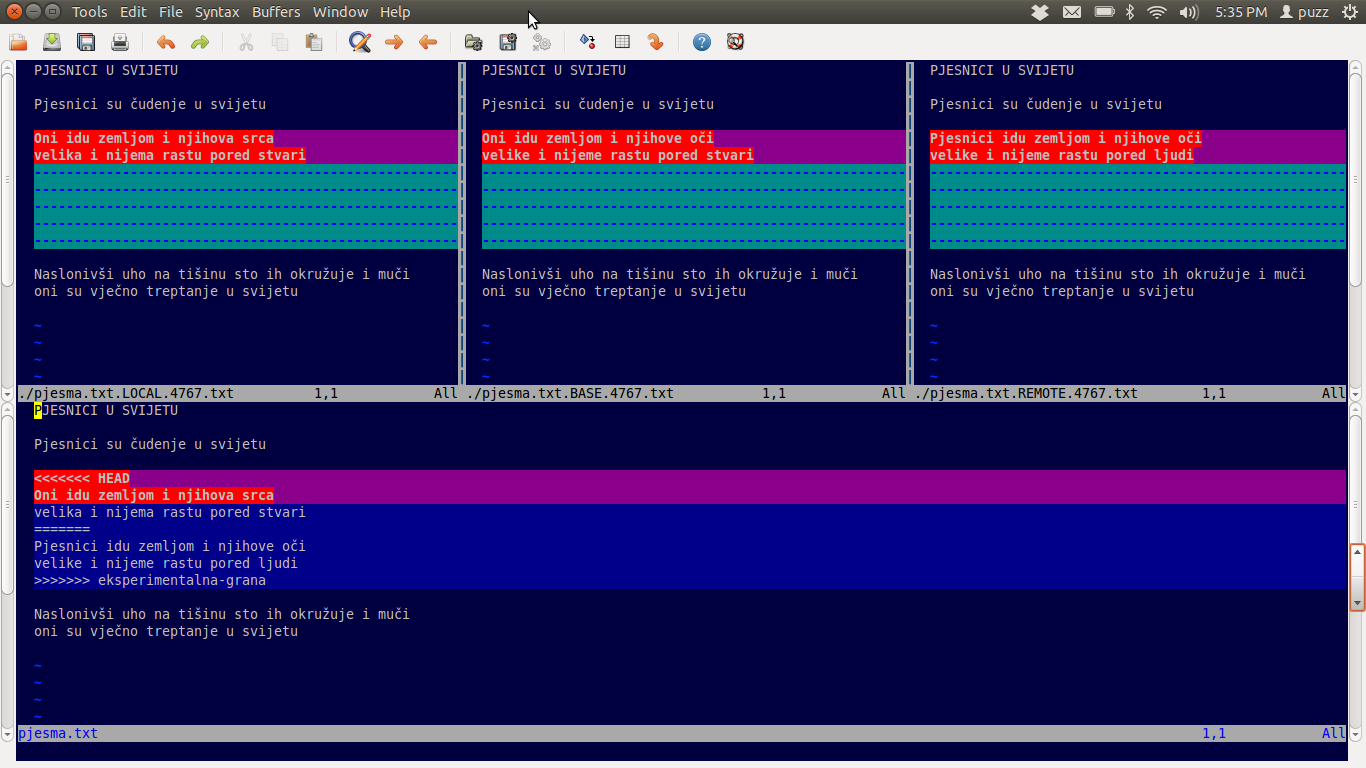
\includegraphics[width=14cm]{images/mergetool.png}

\section*{Merge, branch i povijest projekta}
\addcontentsline{toc}{section}{Merge, branch i povijest projekta}

Kad radimo s nekim projektom, onda nam je uvijek važno da imamo sačuvanu povijest projekta.
To nam omogućava da saznamo tko je originalni autor nekog koda kojeg možda slabije razumijemo.
Ili želimo vidjeti kojim redosljedom je neka datoteka rasla.

Sa standardnim sustavima za verzioniranje, stvar je jednostavna. 
Grananje i preuzimanje izmjena iz jedne u drugu granu je bilo komplicirano i rijetko se radilo. 
Posljedica je da su projekti \emph{uvijek} imali linearnu povijest.

\input{graphs/linearni_model}

S gitom, uvijek se tu nalaze mnoge grane.
Svaka od tih grana ima svoju povijest, a kako se povećava broj grana, tako organizacija projekta postaje veći izazov.
I zato mnogi programeri grane koje više ne koriste brišu.

No, tu sad imamo mali problem.
Pogledajte, na primjer, ovakav projekt:

\input{graphs/git_merge_2}

Eksperimentalna grana ima svoju povijest, a u trenutku \emph{merge}a, sve izmjene iz te grane su se "prelile" u \verb+master+ i to u \emph{commit} \emph d.
Kad bi obrisali \verb+eksperimentalna-grana+ -- izgubili bi cijelu povijest te grane.
Sve međukorake kako je ona nastajala, sve bi nestalo.

Nekome to nije problem, ali desiti će vam se situacija da to ne želite.
Drugim riječim, ne biste htjeli da imate previše grana (jer vam to otežava organizaciju projekta), a ne želite gubiti povijest nastajanja svake od tih grana.
To se može riješiti nečime što se zove \verb+rebase+.
No, da ti to mogli malo bolje objasniti, potrebno je napraviti digresiju u jednu posebnu vrstu \emph{merge}a -- \emph{fast forward}\dots

\section*{Fast forward}
\addcontentsline{toc}{section}{Fast forward}

Nakon objašnjenja s prethodnih nekoliko stranica, trebalo bi biti jasno što će se desiti ako želimo preuzeti izmjene iz \verb+varijanta+ u \verb+master+ u projektu koji ima ovakvu povijest:

\input{graphs/bez_fast_forward}

To je najobičniji \emph{merge} dvije grane.
Razmislimo samo, na trenutak, o jednom očitom detalju;
osnovna pretpostavka i smisao preuzimanja izmjena iz jedne grane u drugu je to što uopće imamo dvije grane.
To su ove dvije crte u gornjem grafu.
Dakle, sve to ima smisla u projektu koji ima nelinearnu povijest (više grana).

No, postoji jedan poseban slučaj koji zahtijeva malo pojašnjenje.
Uzmimo da je povijest projekta bila slična gornjem grafu, ali s jednom malo izmjenom:

\input{graphs/fast_forward}

Programer je napravio novu granu \verb+varijanta+ i na njoj je nastavio rad.
I svo to vrijeme nije radio nikakve izmjene na \verb+master+.
Što kad sad želi preuzeti sve izmjene u \verb+master+?

Uočavate li š1to je ovdje neobično?
Iako imamo dvije grane, \emph{smisao} \emph{merge}anja je u tome da neke izmjene iz jedne grane preuzmemo u drugu.
Međutim, iako ovdje imamo dvije grane, \textbf{one čine jednu crtu}. 
Te dvije grane imaju jednu povijest. 
I to linearnu povijest.

Tako su razmišljali i originalni autori gita.
U git su ugradili automatsko prepoznavanje ovakve situacije i zato, umjesto standardnog \emph{merge}a, koji bi izgledao ovako:

\input{graphs/fast_forward_2}

\dots{}git izvršava takozvani \emph{fast-forward merge}:

\input{graphs/fast_forward_3}

Dakle, doslovno kopira cijelu povijest (ovdje je to \emph x, \emph y i \emph z) u novu granu.
Čak i ako sad obrišete \verb+varijanta+, cijela njega povijest se nalazi u \verb+master+.

Git sam odlučuje je li potrebno izvršiti \emph{fast-forward merge} i izvršava ga. Ukoliko to želite izbjeći -- to se radi tako da dodate opciju \verb+--no-ff+ naredbi \verb+git merge+:

\gitoutputcommand{git merge --no-ff varijanta}

\section*{Rebase}
\addcontentsline{toc}{section}{Rebase}

Po $n$-ti put, pogledajmo linearni model:

\input{graphs/linearni_model}

Do sada bi svima trebalo biti jasno da on ima svoje mane.
No, ima i nešto korisno -- jednostavna i pregledna povijest projekta i privid da je sve skupa teklo po nekom točno određenom rasporedu.
Korak po korak, do trenutne verzije.

Git vas ne tjera da radite grane, no postupak grananja čini bezbolnim. 
U zbog toga povijest projekta \emph{može} postati cirkus kojeg je teško pratiti organizirati.
To zahtijeva malo veću pažnju kad imate puno grana.

Postoji, ipak, način kako se može od puno grana stvoriti linearna povijest.
Kad bi postojao trik kako da iz ovakvog stanja:

\input{graphs/bez_fast_forward}

\dots{}stvorimo ovo:

\input{graphs/bez_fast_forward_rebase}

To jest, da \emph{pomaknemo mjesto od kud smo granali} neku granu. 
Tada bi \emph{fast-forward} samo kopirao cijelu našu granu u \verb+master+.
Kad bi obrisali \verb+varijanta+, povijest bi odjednom postala linerna:

\input{graphs/bez_fast_forward_rebase_2}

Taj trik postoji i zove se \emph{rebase}.

Radi se na sljedeći način; trebate biti postavljeni u grani koju želite "pomaknuti". Onda upišite \verb+git rebase <grana>+, gdje je \verb+<grana>+ ona grana na koju kasnije želite napraviti \emph{fast-forward}. 
Dakle, želite li granu \verb+test+ "pomaknuti" na kraj grane \verb+master+, \emph{rebase} utipkati ćete:

\gitoutputcommand{git rebase master}

U idealnoj situaciji, git će znati riješiti sve probleme i ispis bi mogao izgledati ovako nekako:

\input{git_output/git_rebase}

Međutim, ovdje mogu nastati problemi slični klasičnom \emph{merge}u.
Tako da će se češće dogoditi:

\input{git_output/git_rebase_konflikt}

Idete li pogledati datoteke, vidjeti ćete da je format konfliktne datoteke isti kao kod konflikta pri \emph{merge}u.
I opet, od nas se očekuje da te konflikte riješimo.
Bilo koristeći \verb+git mergetool+, bilo tako da editirate datoteku i ispravite je u željeno stanje. 

Promotrimo još jednom grafički prikaz onoga što ovdje pokušavamo napraviti:

\input{graphs/fast_forward_4}

Naš cilj je preseliti \textcolor{gray}{sivi} tako da postane \textcolor{blue}{plavi}.
Drugim riječim, izmjene koje smo napravili u \emph d, \emph e i \emph f treba nekako "ugurati" prije \emph x, \emph y i \emph z.
I tako ćemo stvoriti novu granu koja se sastoji \emph{x'}, \emph{y'} i \emph{z'}.

Git će automatski napraviti koliko može.
No, kad dođe konflikt (kao što je u primjeru kojeg trenutno obrađujemo), to trebate napraviti vi.

Ako koristite \verb+mergetool+, to ćete izvesti\dots

\input{git_output/git_rebase_konflikt_mergetool}

Važno je napomenuti da, nakon što se konflikt ispravili, \textbf{ne smijete izmjene \emph{commit}ati}, nego samo spremiti u indeks s \verb+git add+.
Nakon toga, utipkajte \verb+git rebase --continue+.
Ponekad će git znati izvršiti ostatak procesa automatski, a može se dogoditi i da ne zna i opet od vas traži da ispravite sljedeći konflikt.
U boljem slučaju (sve automatski), rezultat će biti ovakav:

\input{git_output/git_rebase_konflikt_continue}

Nakon toga, slobodni ste izvesti \emph{merge}, koji će u ovom slučaju sigurno biti \emph{fast-forward}, a to je upravo ono što smo htjeli.

\section*{Rebase ili ne?}
\addcontentsline{toc}{section}{Rebase ili ne?}

Rebase ne morate nužno raditi.
Na vama je odluka želite li izmjene iz neke grane sačuvati u povijesti projekta ili prepustiti zaboravu (za trenutak kad i ako granu obrišete).

Ponekad će vam se dogoditi da sam \emph{rebase} ima previše konflikata pa ćete odustati.
U svakom slučaju, ukoliko ste ga i započeli, uvijek ga možete prekinuti s:

\gitoutputcommand{git rebase --abort}

\section*{Cherry-pick}
\addcontentsline{toc}{section}{Cherry-pick}

Ima još jedna posebna vrsta \emph{merge}a, a nosi malo neobičan naziv \emph{cherry-pick}\footnote{Engleski: branje trešanja. U prenesenom značenju: ispričati priču samo sa onim detaljima koji su pripovjedaču važni. Iliti, izbjegavanje onih dijelova priče koje pripovjedač ne želi.}.

Radi se o sljedećem, zamislite da imate dvije grane:

\input{graphs/git_merge_1}

U \verb+eksperimentalna-grana+ ste nappravili nekoliko izmjena i sve te izmjene \emph{nisu} još spremne da biste ih prebacili u \verb+master+.

Međutim, ima jedan \emph{commit} (recimo da je to \emph g) s kojim ste ispravili mali bug koji se manifestirao i u \verb+master+ grani.
Klasični \emph{merge} oblika:

\input{graphs/git_merge_2}

\dots{}ne dolazi u obzir, jer bi on u \verb+master+ prebacio i sve izmjene koje ste napravili u \emph d, \emph e, \emph f i \emph g.
Mi želimo samo i isključivo \emph g.
To se, naravno, može i to je (naravno) taj \emph{cherry-pick}.

Postupak je sljedeći; prvo pogledajte povijest grane \verb+eksperimentalna-grana+:

\input{git_output/git_log_za_cherry_pick}

Kao što ste vjerojatno već primijetili, svaki \emph{commit} u povijesti ima neki čudan string kao \verb+5c843fbfb09382c272ae88315eea9d77ed699083+.
Taj string jedinstveno određuje svaki \emph{commit} (više riječi o tome u posebnom poglavlju).

Sad trebate naći takav identifikator za onaj commit kojeg želite prebaciti u \verb+master+. Recimo da je to \verb+2b9ef6d02e51a890d508413e83495c11184b37fb+.

Prebacite se u granu u koju želite preuzeti samo izmjene it tog \emph{commit}a i utipkajte \verb+git cherry-pick <commit>+.
Ako nema konflikata, rezultat će biti otprilike:

\input{git_output/git_cherry_pick}

\dots{}a, ako imate konflikata onda\dots

\section*{Merge bez \emph{commit}a}
\addcontentsline{toc}{section}{Merge bez \emph{commit}a}

Vratimo se open na klasični \emph{merge}.
Ukoliko je prošao bez ikakvih problema, onda ćete nakon\dots

\input{graphs/git_merge_2}

\dots{}u povijesti projekta vidjeti nešto kao:

\input{git_output/git_merge_log}

Vratimo se opet na cijelu onu priču oko \emph{rebase}.
Poanta cijele priče je bila u tome što, ako obrišemo granu, brišemo i cijelu njenu povijest.
Ako se već odlučimo da ne želimo \emph{rebase} onda bi bilo lijepo u povijesti projekta umjesto \texttt{Merge branch 'eksperimentalna-grana'} imati smisleniji komentar koji bi bolje opisao što smo točno u toj grani napravili.
Na taj način će, čak i ako granu obrišemo, ostati jedan commit u kojem je opisano što je taj \emph{merge} riješio.

To se može tako da, umjesto \verb+git merge eksperimentalna-grana+ \emph{merge} izvršimo s:

\gitoutputcommand{git merge eksperimentalna-grana --no-commit}

Na taj naćin če se \emph{merge} izvršiti, ali neće se sve \emph{commit}ati. 
Sad vi možete spremiti sve izmjene i staviti neki svoj komentar.

Jedini detalj na kojeg treba pripaziti je što, ako je došlo do \emph{fast-forward} \emph{merge}anja, onda \verb+--no-commit+ nema efekta.
Zato, a za svaki slučaj, je bolje koristiti sljedeću sintaksu:

\gitoutputcommand{git merge eksperimentalna-grana --no-ff --no-commit}
